\section{Search Techniques}
\label{sec:search-techniques}

The second part of solving a program synthesis problem is deciding which search
technique to apply in order to find the intended program.
First, we want to ensure that the program satisfies the semantic and syntactic
specifications.
Second, we want to leverage the specifications and the knowledge we have from
the problem domain in order to guide the search.
Common search techniques are
% deductive search (Section~\ref{sec:deductive-synthesis}),
enumerative search~\cite{Phothilimthana:2016:SUS,Alur:2017:SEP}
(Section~\ref{sec:enumerative-search}),
stochastic search~\cite{Schkufza:2013:SS,Singh:ranking:2015}
(Section~\ref{sec:stochastic-search}), and
constraint solving~\cite{Feng:2018:PSU,Feng:2017:CST,Feng:2017:CSC}
(Section~\ref{sec:constraint-solving}).
Modern synthesizers usually apply a combination of those, enabling us to
consider frameworks and techniques for structuring their construction, such as
\gls{cegis}~\cite{Solar-Lezama:2008},
\gls{cegis}($\mathcal{T}$)~\cite{Abate:2018:CMT}, and
\gls{ogis}~\cite{Jha:2017:TFS}
(Section~\ref{sec:ogis}).


% \subsection{Deductive Synthesis}
\label{sec:deductive-synthesis}

The fundamental idea in deductive synthesis is to extract a program
automatically from the constructive proof of a theorem induced by the
specification. Typically, the kinds of specifications associated with this
method of synthesis are logical relations between inputs and the outputs of the
program. 

These systems tend to require a complete formal specification, and the level
of expertise needed to use them turn them easily unapproachable by the user
which is not mathematically inclined.

\subsection{Enumerative Search}
\label{sec:enumerative-search}

In the context of program synthesis an enumerative search consists of
enumerating programs by working the intrinsic structure of the program space to
guide the search. The programs can be ordered using many different program
metrics, the simplest one being program size~\cite{Alur:sygus:2013}, and pruned
by means of \todo{semantic equivalence checks}{Missing an example to explain
what I mean. Maybe add a simple example such as, how by associativity of
addition, x+y is the same as y+x} with respect to the specification.
Synthesizers based on enumerative search haven been some of the most effective
to synthesize short programs in complex program spaces~\cite{Gulwani2017}.

A simple enumerative search algorithm is described in Figure \fixme{???}{ainda
tenho que produzir esta figura}. The algorithm is parameterized by the
specification $\phi{}$ and two procedures, $next$, that given a set of programs
generates a new set of programs, and $prune$, that given a set of programs
filters out the \todo{unwanted ones}{Isto poderia ser dito de uma outra
forma...}. The algorithm works by iteratively calling the given procedures until
it finds a program that matches the specification.

In their overview of the field of program synthesis~\cite{Gulwani2017},
\citeauthor{Gulwani2017} present some simple enumerative search algorithms for
finding programs in program spaces defined by a \gls{cfg}, which we describe
next. The algorithms can be generalized to other types of program spaces such
as, e.g., partial programs.

\subsubsection{Top-Down Tree Search}
\label{sec:top-down-tree-search}

The first algorithm, shown in Figure \fixme{?}{ainda tenho que produzir esta
figura.}, takes as input a \gls{cfg} $G = (V, \Sigma{}, R, S)$ and a
specification $\phi{}$, and works by exploring the derivations of $G$ in a
top-down fashion. The algorithm stores the current programs in a priority queue,
$P$, and stores all the programs found so far in the set $P'$. Both $P$ and $P'$
are initialized with the partial program that corresponds to the start symbol
$S$ of $G$. The algorithm runs until it finds a program $p$ that matches the
specification $\phi{}$ or there are no more programs waiting in the queue
(meaning that the algorithm fails). At every iteration, we take the highest
priority program $p$ from the queue and check whether it satisfies $\phi{}$. If
yes, we return $p$. Otherwise, the algorithm finds new (possibly partial)
programs by applying the production rules of the grammar to $p$. The program
space is pruned in the next step by ignoring programs that are semantically
equivalent with respect to $\phi{}$ to programs already considered in the past
($P'$).

% TODO: Adicionar (possivelmente) um exemplo de um traço de execução do
% algoritmo.

\subsubsection{Bottom-Up Tree Search}
\label{sec:bottom-up-tree-search}

The second algorithm, shown in Figure \fixme{?}{ainda tenho que produzir esta
figura.}, also takes a \gls{cfg} $G = (V, \Sigma{}, R, S)$ and a specification
$\phi{}$, and works by exploring the derivations of the grammar in a bottom-up
dynamic programming fashion. This strategy has the advantage over the top-down
search that (in general) only complete programs may be evaluated for semantic
equivalence. The algorithm maintains a set of semantically equivalent
expressions, first considering the programs corresponding to leafs of the syntax
tree of the grammar $G$, and then composing them in order to build expressions
of increasing complexity, essentially applying the rules of the grammar in the
opposite direction.

% TODO: Check out references [4, 141] of Gulwani2017.

% This algorithm is shown in Figure \fixme{???}{ainda tenho que produzir esta
% figura}, using program size as the metric of program complexity.

\subsubsection{Bidirectional Tree Search}
\label{sec:bidirectional-search}

We can see that a top-down tree search starts from a set of input states, while
a bottom-up tree search starts from a set of output states. The third algorithm,
shown in Figure \fixme{?}{ainda tenho que produzir esta figura.}, combines the
previous two approaches, starting from both a set of input states and a set of
output states. It maintains both sets, evolving in the same way the previous two
algorithms did and stopping when it finds a state that belongs to both sets in a
sort of meet-in-the-middle approach.

% TODO: Explicar porque que isto e bom.
% Note that instructions _ and _ may be parallelizable.
\subsection{Stochastic Search}
\label{sec:stochastic-search}

Stochastic search is an approach to program synthesis where the synthesizer uses
probabilistic reasoning to learn a program conditioned on the specification. Two
typical approaches to applying stochastic search in synthesizers are as follows.
One is to learn a \textit{guiding function} that works on top of an enumerative
search algorithm to help it predict which program from the search space is most
likely to meet the desired specification. Another one is to learn a probability
distribution over the search space in order to sample programs that are more
promising. Below, we can find high-level descriptions of specific instances of
these kinds of synthesis.

\subsubsection{Guiding the Search}
\label{sec:guiding}

\subsubsection{Sampling the Search Space}
\label{sec:sampling}

In this section we describe the stochastic synthesizer used by
\citeauthor{Alur:sygus:2013} in their syntax-guided synthesis
paper~\cite{Alur:sygus:2013}. Their synthesizer learns from examples and is
adapted from work on superoptimization of loop-free binary
programs~\cite{Schkufza:2013:SS}. They define a score function, $Score$, that
measures the extent which a given program is consistent with the specification.
Then they perform a probabilistic walk over the search space while maximizing
this score function. The algorithm works by first picking a program $p$ of fixed
size $n$ uniformly at random. They then pick a node from its parse tree
uniformly at random and consider the subprogram rooted at that node. They then
substitute it with another subprogram of same size and type, chosen uniformly at
random, obtaining a new program $p'$. The probability of discarding $p$ for $p'$
is given by the formula $min(1, Score(p')/Score(p))$. It remains to say how to
pick the value of $n$. Typically we do not know the size of the desired program
from the start. In order to tackle this problem, they start by fixing its value
at $n = 1$ and at each iteration change its value to $min(1, n\pm{}1)$ with with
some small probability (default is 0.01).

\subsection{Constraint Solving}
\label{sec:constraint-solving}

% TODO: Check out 132, 133, 134 of the overview

Another approach to program synthesis is to reduce the problem to that of
constraint solving by the use of off-the-shelf automated constraint
solvers~\cite{Shi:2019:FCS,Feng:2018:PSU,Feng:2017:CST,Feng:2017:CSC,Solar-Lezama:2008,Jha:oracle:2010}
(typically SAT or SMT solvers).

% TODO: Propositional formulas, SAT, SMT, LIA and simple encoding examples --> preliminaries

One idea is to encode the specification in a logical constraint whose solution
corresponds to the desired program. \citeauthor{Gulwani2017} illustrate this
idea nicely with an example~\cite{Gulwani2017} which we adapt here.
Suppose our programs are composed of operations over two input bitvectors, $x$
and $y$ of length eight:

% FIXME
\begin{figure}[h!]
  \centering
  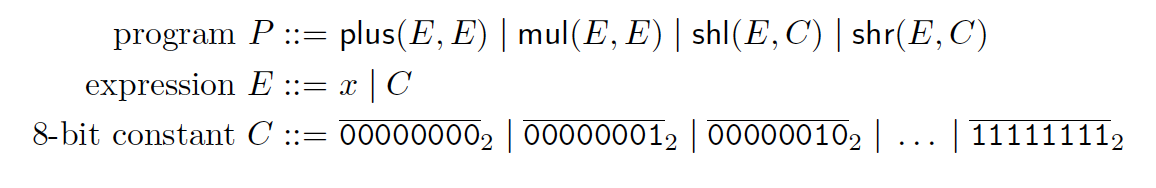
\includegraphics[width=\textwidth]{assets/constraint-solving-example.png}
  \caption{FIXME: This example is a placeholder and should be adapted.}
\end{figure}

We consider an expression to be the input variable $x$ or an 8-bit constant. A
program consists of additions and multiplications between expressions, or of
shift left/right operations over an expression by a constant.

Imagine we are interested in a program that \todo{<insert interesting bit
  twiddling hack>}{check Hacker's Delight}. In the theory of
\todo{bitvectors}{missing ref}, the program we are interested in can be encoded
by the formula \todo{<insert formula here>}{add formula correspondent to the
hack}. To find the program we can write the constraints in the SMT-LIB format
and feed them to an SMT solver:

% FIXME
\begin{figure}[h!]
  \centering
  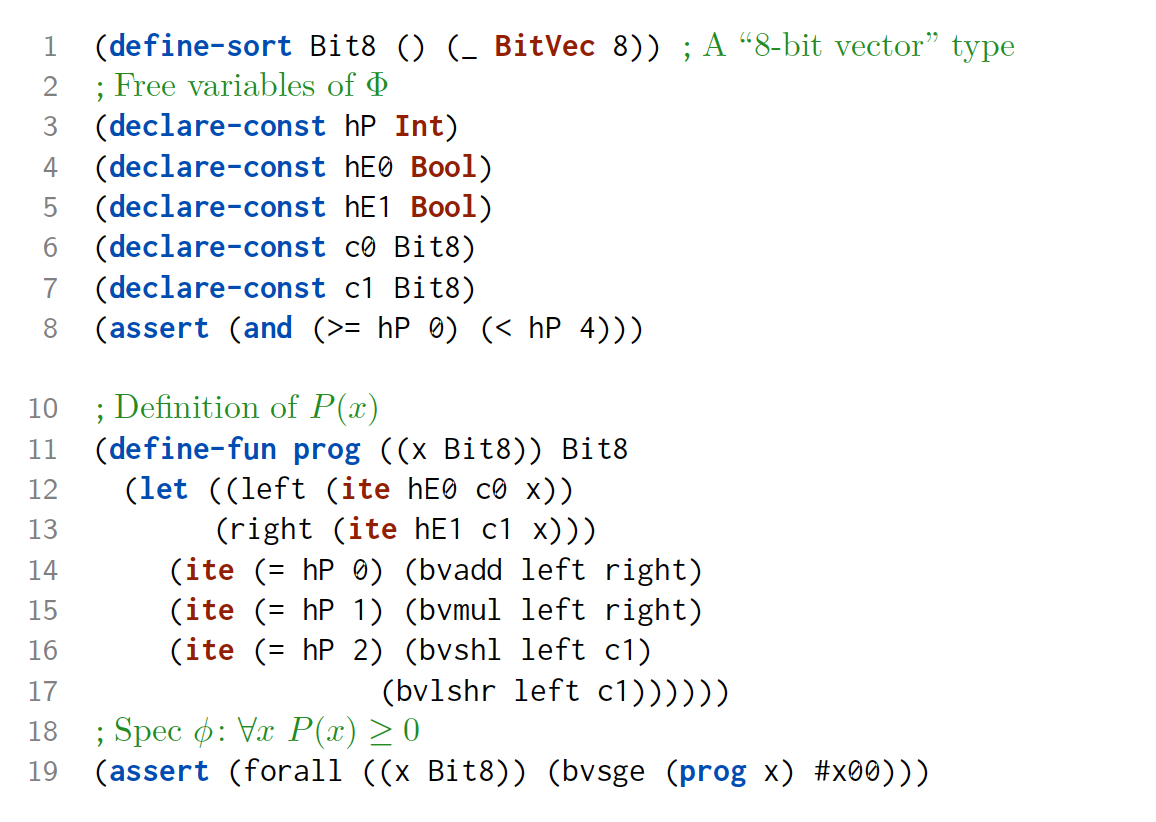
\includegraphics[width=\textwidth]{assets/constraint-solving-smtlib.png}
  \caption{FIXME: This example is a placeholder and should be adapted.}
\end{figure}

This example shows an end-to-end constraint solving approach to program
synthesis. However, enconding the problem this way can sometimes be non-trivial
or time-consuming. This idea led to the appearance of the concept of
\textit{solver-aided programming}, where programming languages are enlarged with
high-level constructs that give the user access to synthesis without having to
deal with the constraint solvers directly.

For example, \citeauthor{Gulwani2017} describe the SKETCH system as a ``compiler
[that] relies on a SAT solver to materialize some language constructs''.
ROSETTE~\cite{Torlak:2013:GSL} is a framework for developing solver-aided
programming languages embedded in Racket that provides constructs not only for
synthesis, but also for verification, debugging and angelic execution.
% SMTEN?
% Metasketching, symbolic profiling?

\subsubsection{Component-Based Synthesis}
\label{sec:components}

% TODO Check
% 12, 13, 22, 34 of Gulwani2017
% 9, 16, 17 of Feng:2017:CSC

One area of program synthesis where constraint solving techniques have seen
considerable use is that of \textit{component-based
synthesis}~\cite{Shi:2019:FCS,Feng:2018:PSU,Feng:2017:CST,Feng:2017:CSC,Jha:oracle:2010}.
In component-based synthesis we are interested in finding a loop-free program
made out of a combination of fundamental building blocks called
\textit{components}. These components could be, for example, methods in a
library \gls{api}~\cite{Shi:2019:FCS,Feng:2017:CSC}, and they form the syntactic
bias for the programs we want to find. They may also be supplemented by
additional constraints in the form of logical formulas~\cite{Feng:2018:PSU}.

% TODO Examples: SyPet and FrAngel
% Also, FrAngel adds control structures to the problem

% TODO
% - Conflict-driven, distinguishing inputs
% - Inductive Logic Programming


\subsection{Oracle-Guided Inductive Synthesis}
\label{sec:ogis}

\textit{\Gls{ogis}} is an approach to program synthesis where the synthesizer is
split into two components: the \textit{learner} and the \textit{oracle}. The two
components communicate in an iterative \textit{query/response} cycle, as shown
in Figure~\ref{fig:ogis}. The learner implements the search strategy to
find the program and is parameterized by some form of program specification
and/or syntactic bias (see~\ref{sec:specifications}). The usefulness of the
oracle is defined by the type of queries it can handle and the properties of its
responses. The characteristics of these components are typically imposed by the
\todo{application}{give an example}.

\begin{figure}[htb]
  \centering
  \begin{tikzpicture}
    [semithick, >=stealth, auto,
     rectangular/.style={rectangle, draw, rounded corners, text width=4cm,
       align=center, minimum size=1.5cm},
     spherical/.style={circle, draw, text width=2cm, align=center}]

    \node [rectangular] (S)  {Learner};
    \node [left=1.95cm of S, align=center] (I) {Specification\\and/or Syntactic Bias}
      edge [->] (S);
    \node [below=of S, align=center] {Program $p$\\or Fail}
      edge [<-] (S);
    \node [spherical] (V)  [right=3cm of S] {Oracle}
      ([yshift=0.2cm]S.east) edge [->, bend left]  node        {Query}    ([yshift=0.2cm]V.west)
      ([yshift=-.2cm]S.east) edge [<-, bend right] node [swap] {Response} ([yshift=-.2cm]V.west);
  \end{tikzpicture}
  \caption{\Acrlong{ogis}. Adapted from
    \protect\citeauthor{Jha:2017:TFS}~\protect\cite{Jha:2017:TFS}.}
  \label{fig:ogis}
\end{figure}

Typical queries and response types are some of the following~\cite{Jha:2017:TFS}:

\begin{itemize}
\item \textit{Membership queries}, where given an I/O example $x$ the oracle
  responds with the answer to whether $x$ is positive or not.
\item \textit{Positive (resp. negative) witness queries}, where the oracle
  responds with a positive (resp. negative) I/O example, if it can find any, or
  $\bot$ otherwise.
\item \textit{Counterexample queries}, where given a candidate program $p$ the
  oracle responds with a positive I/O counterexample that $p$ does not satisfy,
  if it can find any, or $\bot$ otherwise.
\item \textit{Correctness queries}, where given a candidate program $p$ the
  oracle responds with the answer to whether $p$ is correct or not. If it is not,
  the oracle responds with a positive I/O counterexample.
\item \textit{Verification queries}, where given program $p$ and specification
  $\phi$ the oracle responds with the answer to whether $p$ satisfies $\phi$ or
  not, or $\bot$ if it cannot find the answer.
\item \textit{Distinguishing input queries}, where given program $p$ and set $X$
  of I/O examples that $p$ \todo{satisfies}{did I define what satisfying a set of
    examples means?} the oracle responds with a new program $p'$ and a
  counterexample $x$ to $p$ that $p'$ satisfies along with all the other
  examples in $X$.
\end{itemize}
% TODO: Maybe switch to ''Jha et al.'s distinguishing inputs`'?
% FIXME: Is this ^^^ too close to the original?

An \gls{ogis} system responding to counterexample queries corresponds to the
\textit{\gls{cegis}} system, introduced by \citeauthor{Solar-Lezama:2008}
~\cite{Solar-Lezama:2008} in the context of the SKETCH synthesizer. Correctness
oracles are more powerful than counterexample oracles because they are
guaranteed to return a counterexample if the program is not correct, where the
counterexample oracles might not.

The concept of \gls{ogis} and distinguishing inputs were introduced by Jha et.
al \cite{Jha:2017:TFS} as a generalization of \gls{cegis} when they applied
this idea in a example-based synthesizer in order to deobfuscate malware and to
generate bit-manipulating programs. Jha et al. further developed this idea by
presenting a new theoretical framework for inductive synthesis
\cite{Jha:2017:TFS}.

\fixme{Aqui tenho dúvida se devo ou não colocar pseudocódigo do algoritmo deles
(Como na figura 3.3. da overview) Ou se já é aprofundar demais. Note que eles
\textbf{não} fazem queries ao utilizador}{}

In general, the higher the capabilities of the oracles, the more expensive they
are to run. Distinguishing oracles are (typically) not as strong as
counterexample or correctness oracles as the returned counterexample is not
necessarily positive. To see why they might by such effectives tools we can
recur to the \todo{Bounded Observation Hypothesis}{caps?} \fixme{first
introduced}{as far as I know} by Solar-Lezama \cite{Solar-Lezama:2008}, which
asserts that ``an implementation that works correctly for the common case and
for all the different corner cases is likely to work correctly for all inputs.''

In a setting of \todo{interactive program synthesis}{defined?} we could see the
users take the role of the oracles. However, the interesting cases are the ones
where the ratio between the amount of work the users are given and the
information given to the synthesizer is maximized. A system that frequently
queries the users for correctness checks would probably feel very cumbersome. On
the other hand, a system that queries for membership or positiveness checks
might be more realistic, as usually the \todo{users}{sometimes I refer to the
user in the singular and sometimes not. I probably should be paying more
attention to this.} have an idea of what sort of examples fit their desired
model.



